%%%%%%%%%%%%%%%%%%%%%%%%%%%%%%%%%%%%%%%%%
% Short Sectioned Assignment LaTeX Template Version 1.0 (5/5/12)
% This template has been downloaded from: http://www.LaTeXTemplates.com
% Original author:  Frits Wenneker (http://www.howtotex.com)
% License: CC BY-NC-SA 3.0 (http://creativecommons.org/licenses/by-nc-sa/3.0/)
%%%%%%%%%%%%%%%%%%%%%%%%%%%%%%%%%%%%%%%%%

%----------------------------------------------------------------------------------------
%	PACKAGES AND OTHER DOCUMENT CONFIGURATIONS
%----------------------------------------------------------------------------------------

\documentclass[paper=a4, fontsize=11pt]{scrartcl} % A4 paper and 11pt font size

% ---- Entrada y salida de texto -----

\usepackage[T1]{fontenc} % Use 8-bit encoding that has 256 glyphs
\usepackage[utf8]{inputenc}
%\usepackage{fourier} % Use the Adobe Utopia font for the document - comment this line to return to the LaTeX default

% ---- Idioma --------

\usepackage[spanish, es-tabla]{babel} % Selecciona el español para palabras introducidas automáticamente, p.ej. "septiembre" en la fecha y especifica que se use la palabra Tabla en vez de Cuadro

% ---- Otros paquetes ----

\usepackage[hidelinks]{hyperref} % Estilo para los enlaces
\hypersetup{
  colorlinks   = true, %Colours links instead of ugly boxes
  urlcolor     = blue, %Colour for external hyperlinks
  linkcolor    = black, %Colour of internal links
  citecolor   = blue %Colour of citations
}
\usepackage{url} % ,href} %para incluir URLs e hipervínculos dentro del texto (aunque hay que instalar href)
\usepackage{amsmath,amsfonts,amsthm} % Math packages
%\usepackage{graphics,graphicx, floatrow} %para incluir imágenes y notas en las imágenes
\usepackage{graphics,graphicx, float} %para incluir imágenes y colocarlas
\usepackage{eurosym}

% Para hacer tablas comlejas
%\usepackage{multirow}
%\usepackage{threeparttable}

%\usepackage{sectsty} % Allows customizing section commands
%\allsectionsfont{\centering \normalfont\scshape} % Make all sections centered, the default font and small caps

\usepackage{fancyhdr} % Custom headers and footers
\pagestyle{fancyplain} % Makes all pages in the document conform to the custom headers and footers
\fancyhead{} % No page header - if you want one, create it in the same way as the footers below
\fancyfoot[L]{} % Empty left footer
\fancyfoot[C]{} % Empty center footer
\fancyfoot[R]{\thepage} % Page numbering for right footer
\renewcommand{\headrulewidth}{0pt} % Remove header underlines
\renewcommand{\footrulewidth}{0pt} % Remove footer underlines
\setlength{\headheight}{13.6pt} % Customize the height of the header

\numberwithin{equation}{section} % Number equations within sections (i.e. 1.1, 1.2, 2.1, 2.2 instead of 1, 2, 3, 4)
\numberwithin{figure}{section} % Number figures within sections (i.e. 1.1, 1.2, 2.1, 2.2 instead of 1, 2, 3, 4)
\numberwithin{table}{section} % Number tables within sections (i.e. 1.1, 1.2, 2.1, 2.2 instead of 1, 2, 3, 4)

\setlength\parindent{0pt} % Removes all indentation from paragraphs - comment this line for an assignment with lots of text

\newcommand{\horrule}[1]{\rule{\linewidth}{#1}} % Create horizontal rule command with 1 argument of height


%----------------------------------------------------------------------------------------
%	TÍTULO Y DATOS DEL ALUMNO
%----------------------------------------------------------------------------------------

\title{	
\normalfont \normalsize 
\textsc{\textbf{Ingeniería de Servidores (2016-2017)} \\ Grado en Ingeniería Informática \\ Universidad de Granada} \\ [25pt] % Your university, school and/or department name(s)
\horrule{0.5pt} \\[0.4cm] % Thin top horizontal rule
\huge Memoria Práctica 4 \\ % The assignment title
\horrule{2pt} \\[0.5cm] % Thick bottom horizontal rule
}

\author{Elena María Gómez Ríos} % Nombre y apellidos

\date{\normalsize\today} % Incluye la fecha actual

%----------------------------------------------------------------------------------------
% DOCUMENTO
%----------------------------------------------------------------------------------------

\begin{document}

\maketitle % Muestra el Título

\newpage %inserta un salto de página

\tableofcontents % para generar el índice de contenidos

\listoffigures

\listoftables

\newpage

%\textbf{NOTA: en caso de problema al compilar, compruebe que tiene el paquete: texlive-babel-spanish.noarch }  \\
 


\newpage

%----------------------------------------------------------------------------------------
%	Cuestión 1
%----------------------------------------------------------------------------------------

\section{Cuestión 1:}

\subsection{a) ¿Seleccione, instale y ejecute uno, comente los resultados. Atención: no es lo mismo un benchmark que una suite, instale un benchmark.}

Para instalar Phoronix Suite en CentOS \cite{phoronix} se utiliza el comando  \texttt{yum install \\ phoronix-test-suite} (figura \ref{fig:ejercicio1_1}). Con el comando \texttt{phoronix-test-suite list-tests} se obtiene una lista de los benchmarks disponibles (figura \ref{fig:ejercicio1_2}). Para intalar un benchmark de la lista se utiliza el comando \texttt{phoronix-test-suite install <test>} (figura \ref{fig:ejercicio1_3}).

La documentación utilizada para los comandos de phoronix ha sido \cite{phoroniComandos}, aunque podemos obtener la misma información con \texttt{man phoronix-test-suite}.\\

Podemos iniciar el cliente web con el comando \texttt{phoronix-test-suite gui} (figura \ref{fig:ejercicio1_4}), el cual abrirá una nueva ventana como se muestra en la figura \ref{fig:ejercicio1_5} en la que aparece la monitorización de nuestro sistema. Desde aquí también podemos listar los test disponibles (figura \ref{fig:ejercicio1_6}) e instalarlos. En la pestaña de ``Installed Tests'' podemos ver los benchmarks ya instalados, en mi caso, como se muestra en la figura \ref{fig:ejercicio1_7}, aparece el ``Blender'' que es el benchmark que he instalado anteriormente.\\

Ejecutar el bechmark desde la GUI es muy sencillo, simplemente debemos pulsar sobre el bechmark que queremos ejecutar y nos saldrá una pantalla como la de la figura \ref{fig:ejercicio1_8}, si el benchmark no está instalado se instalará previamente. Mientras que se ejecuta el benchmark se muestra la siguiente pantalla de información, figura \ref{fig:ejercicio1_9}, donde informa del tiempo aproximado que va a tardar en completarse.\\

Debido a que mi máquina virtual no es capaz de finalizar el benchmark de Blender, he decidido cancelar la ejecución tras unos 46 minutos (figura \ref{fig:ejercicio1_10}) y probar con otro que requiera menos requisitos y tarde menos en finalizar la ejecución, como por ejemplo ``GLmark2'' (figura \ref{fig:ejercicio1_11} y \ref{fig:ejercicio1_12}).\\

Una vez finalizado el benchmark de ``GLmark2'', como se muestra en la figura \ref{fig:ejercicio1_13}, accedemos a los resultados donde podemos ver un listado de las especificaciones de nuestro sistema y una puntuación del test realizado(figuras \ref{fig:ejercicio1_14} y \ref{fig:ejercicio1_15}).



\begin{figure}[H] 
	\centering
	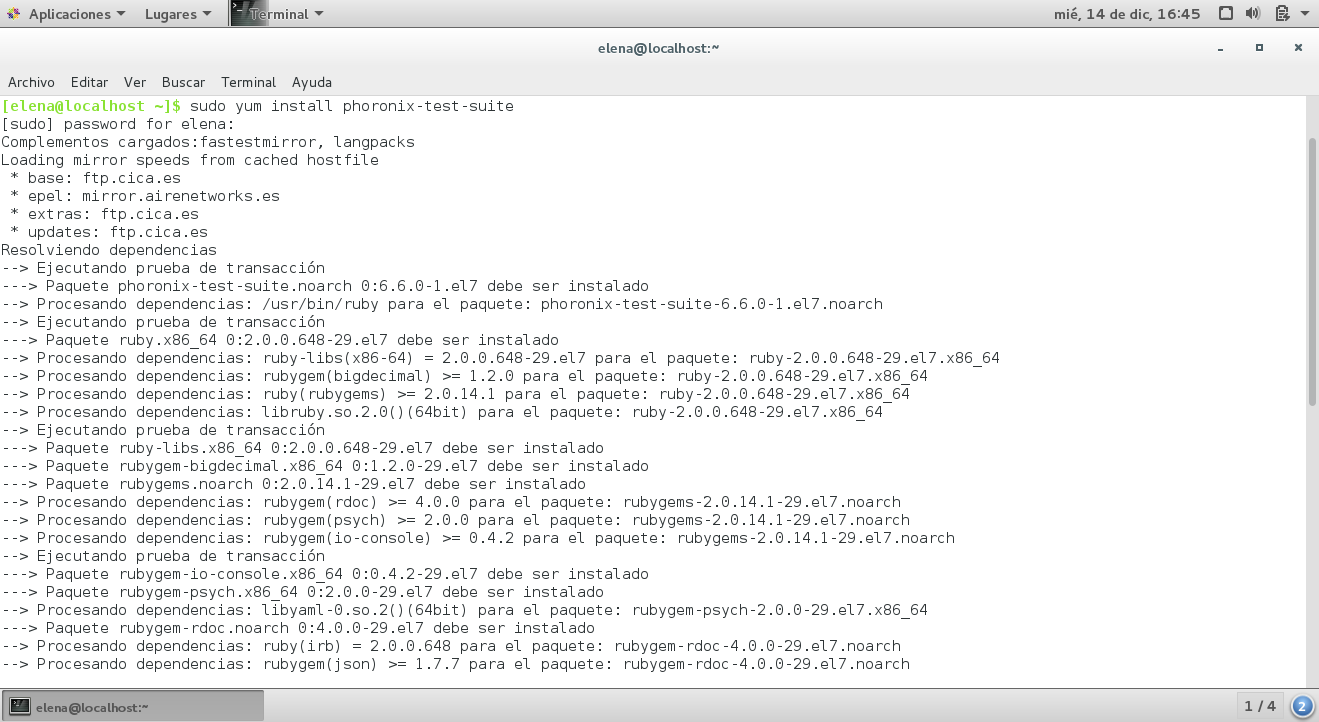
\includegraphics[width=14.7cm]{./img/ejercicio1_1.png} 	
	\caption{CentOS, instalación de Phoronix Suite.} \label{fig:ejercicio1_1}
\end{figure}

\begin{figure}[H] 
	\centering
	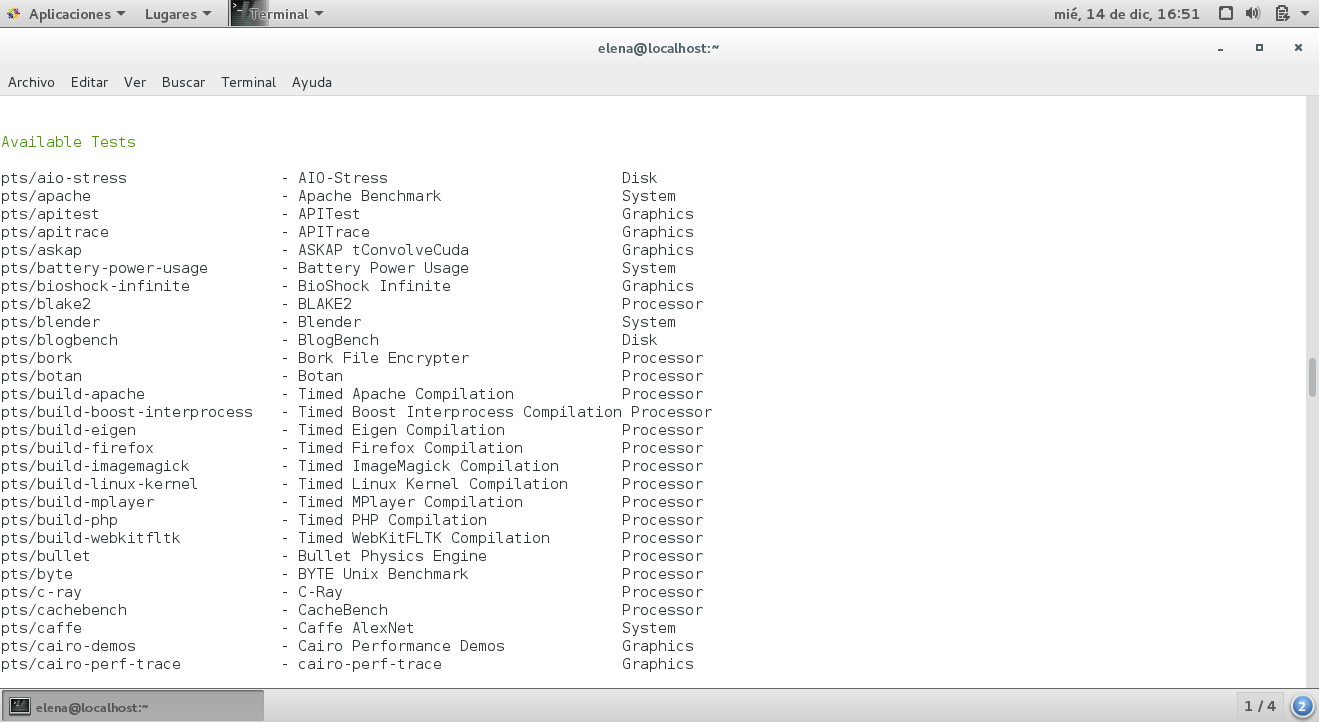
\includegraphics[width=14.7cm]{./img/ejercicio1_2.png} 	
	\caption{CentOS, listado de benchmarks.} \label{fig:ejercicio1_2}
\end{figure}

\begin{figure}[H] 
	\centering
	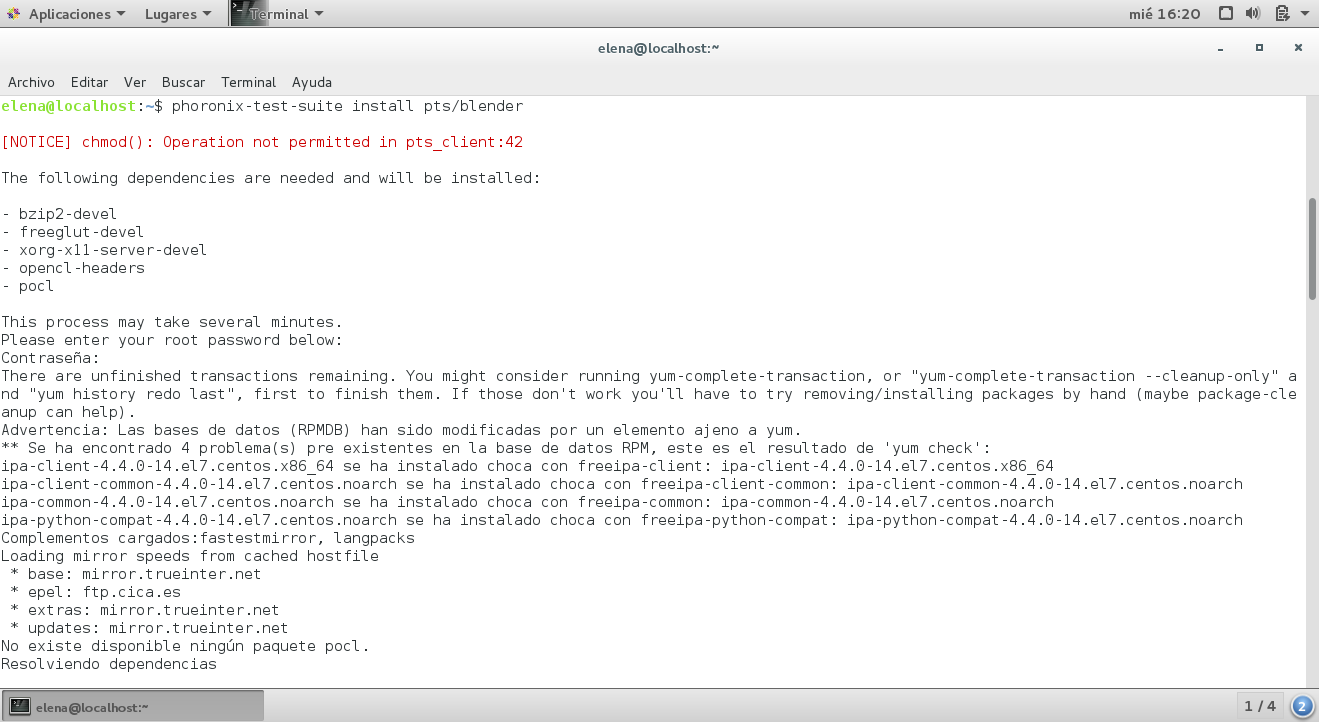
\includegraphics[width=14.7cm]{./img/ejercicio1_3.png} 	
	\caption{CentOS, instalación del benchmark Blender.} \label{fig:ejercicio1_3}
\end{figure}

\begin{figure}[H] 
	\centering
	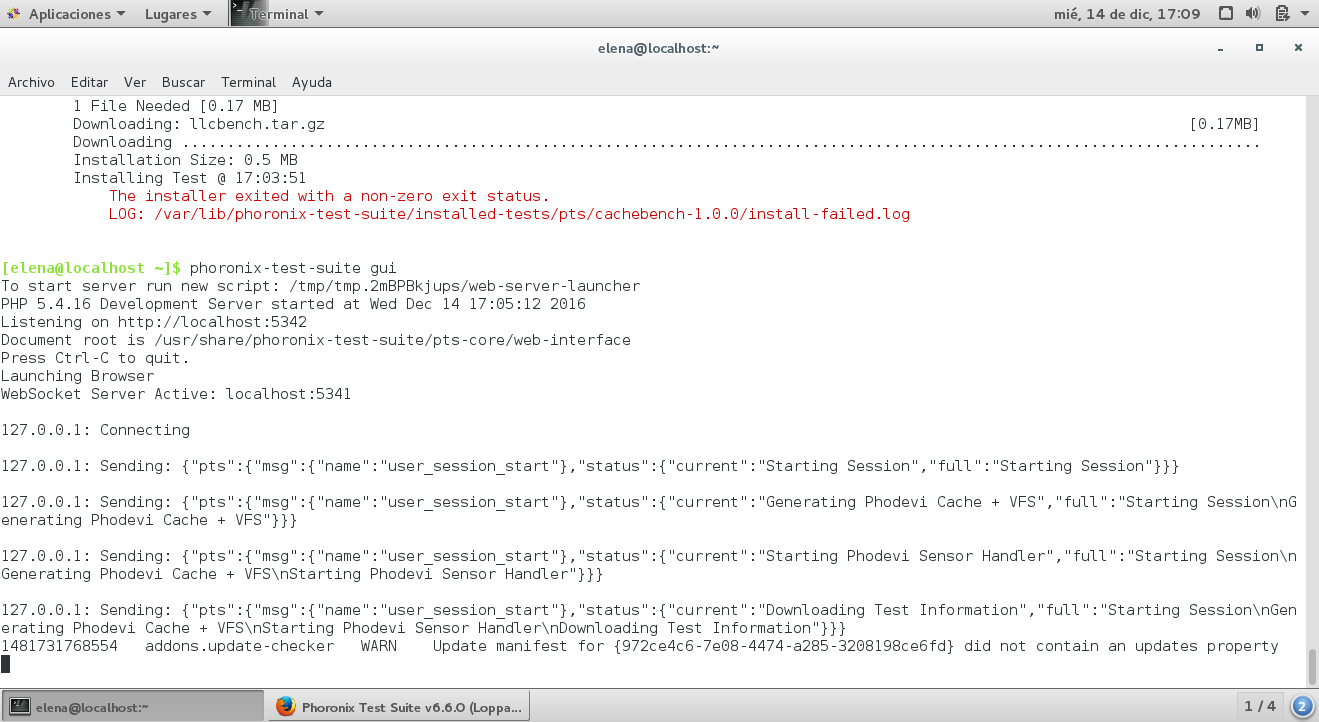
\includegraphics[width=14.7cm]{./img/ejercicio1_4.png} 	
	\caption{CentOS, Phoronix Suite GUI.} \label{fig:ejercicio1_4}
\end{figure}

\begin{figure}[H] 
	\centering
	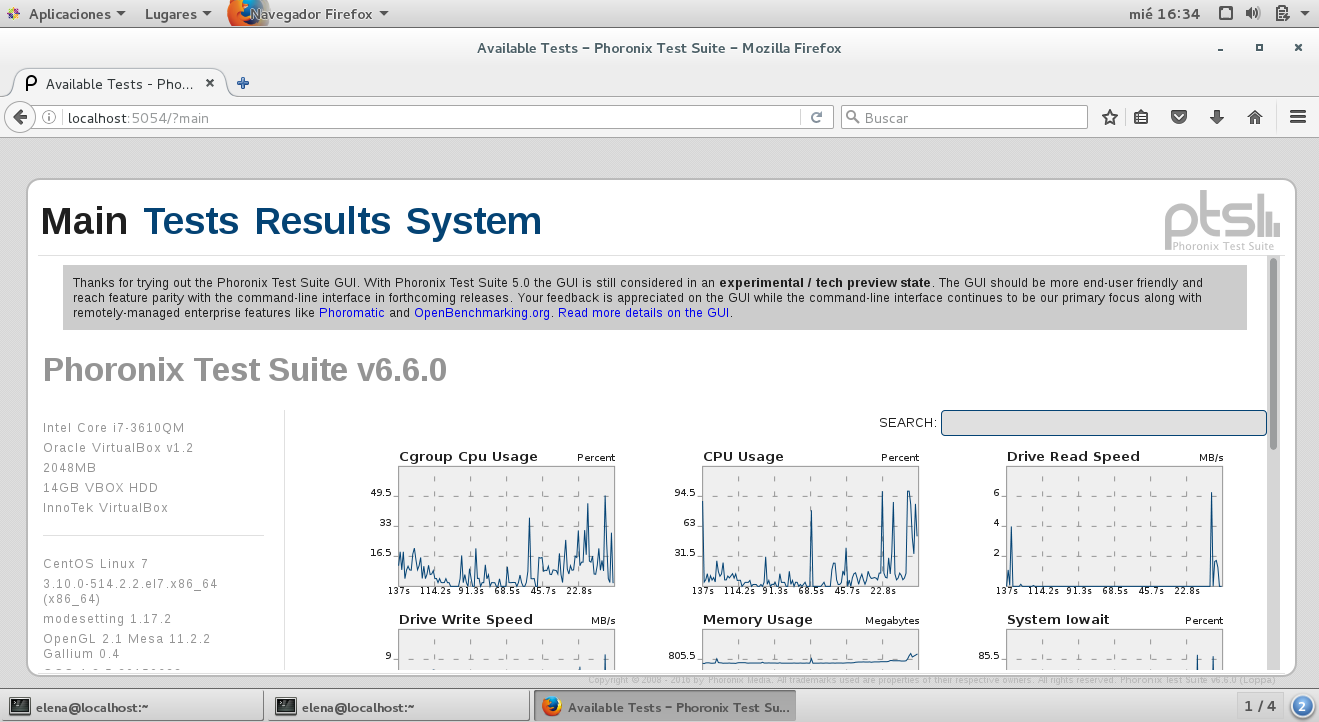
\includegraphics[width=14.7cm]{./img/ejercicio1_5.png} 	
	\caption{CentOS, Phoronix Suite GUI web.} \label{fig:ejercicio1_5}
\end{figure}

\begin{figure}[H] 
	\centering
	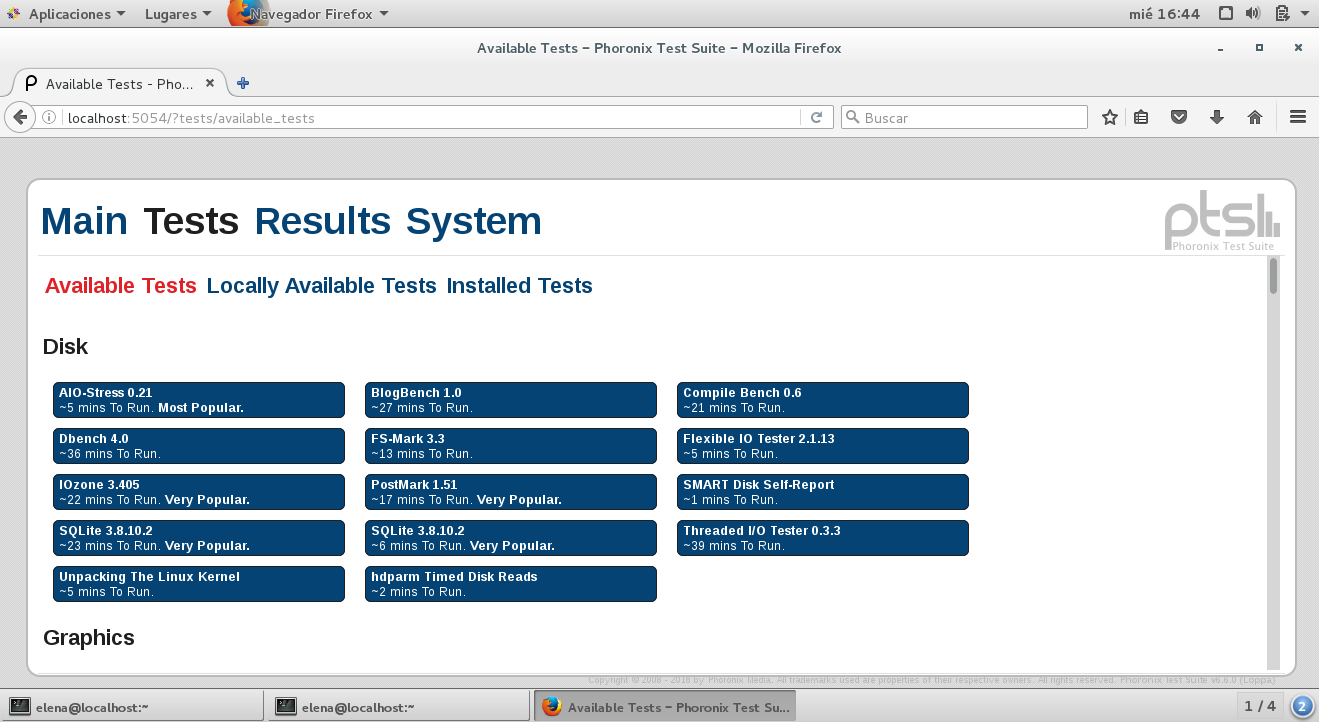
\includegraphics[width=14.7cm]{./img/ejercicio1_6.png} 	
	\caption{CentOS, Phoronix Suite, listado de benchmarks.} \label{fig:ejercicio1_6}
\end{figure}

\begin{figure}[H] 
	\centering
	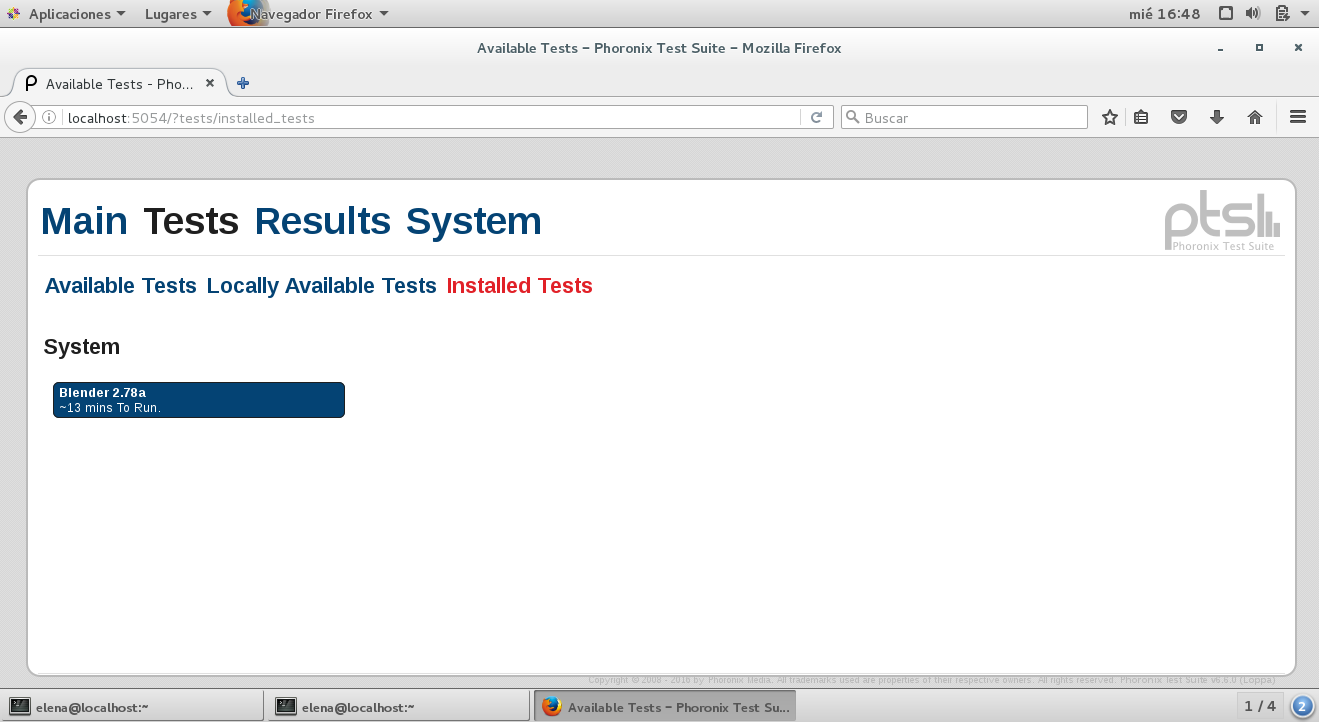
\includegraphics[width=14.7cm]{./img/ejercicio1_7.png} 	
	\caption{CentOS, Phoronix Suite, listado de benchmarks instalados.} \label{fig:ejercicio1_7}
\end{figure}

\begin{figure}[H] 
	\centering
	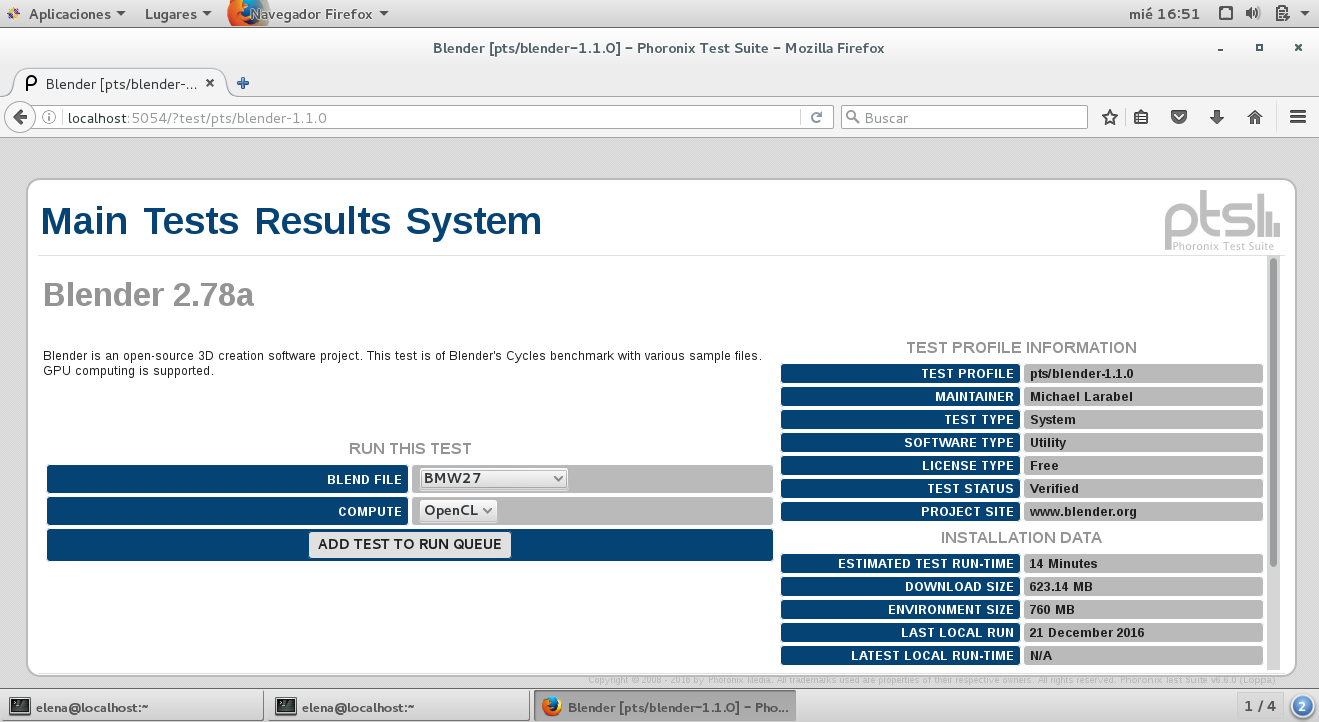
\includegraphics[width=14.7cm]{./img/ejercicio1_8.png} 	
	\caption{CentOS, Phoronix Suite, ejecución de benchmarks.} \label{fig:ejercicio1_8}
\end{figure}

\begin{figure}[H] 
	\centering
	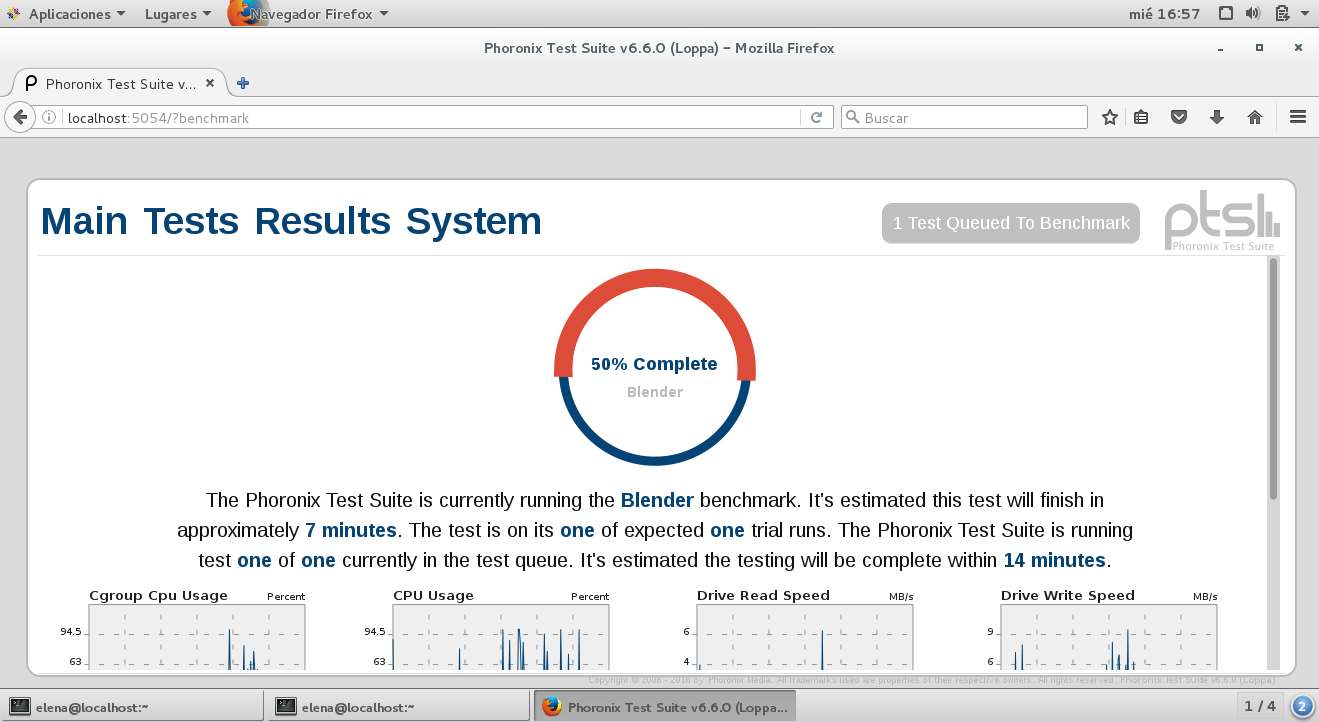
\includegraphics[width=14.7cm]{./img/ejercicio1_9.png} 	
	\caption{CentOS, Phoronix Suite, ejecución de benchmarks.} \label{fig:ejercicio1_9}
\end{figure}

\begin{figure}[H] 
	\centering
	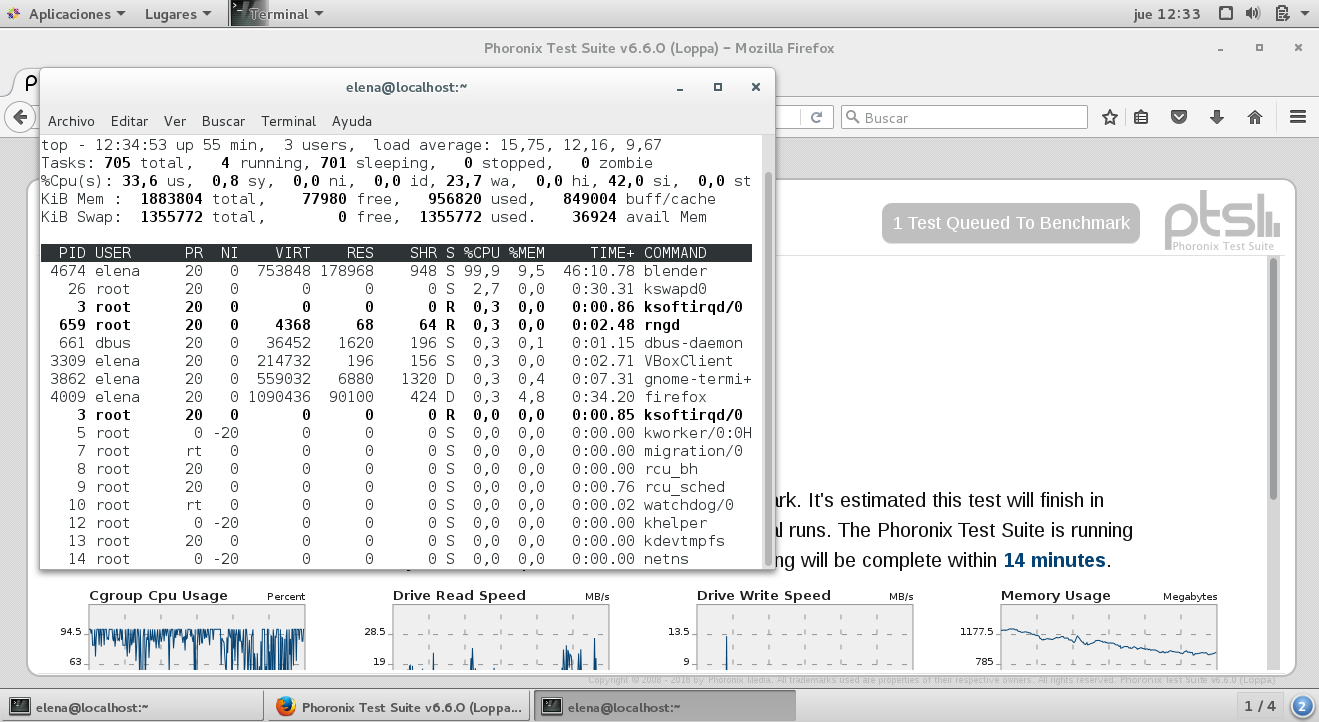
\includegraphics[width=14.7cm]{./img/ejercicio1_10.png} 	
	\caption{CentOS, Phoronix Suite, problemas con benchmark Blender.} \label{fig:ejercicio1_10}
\end{figure}

\begin{figure}[H] 
	\centering
	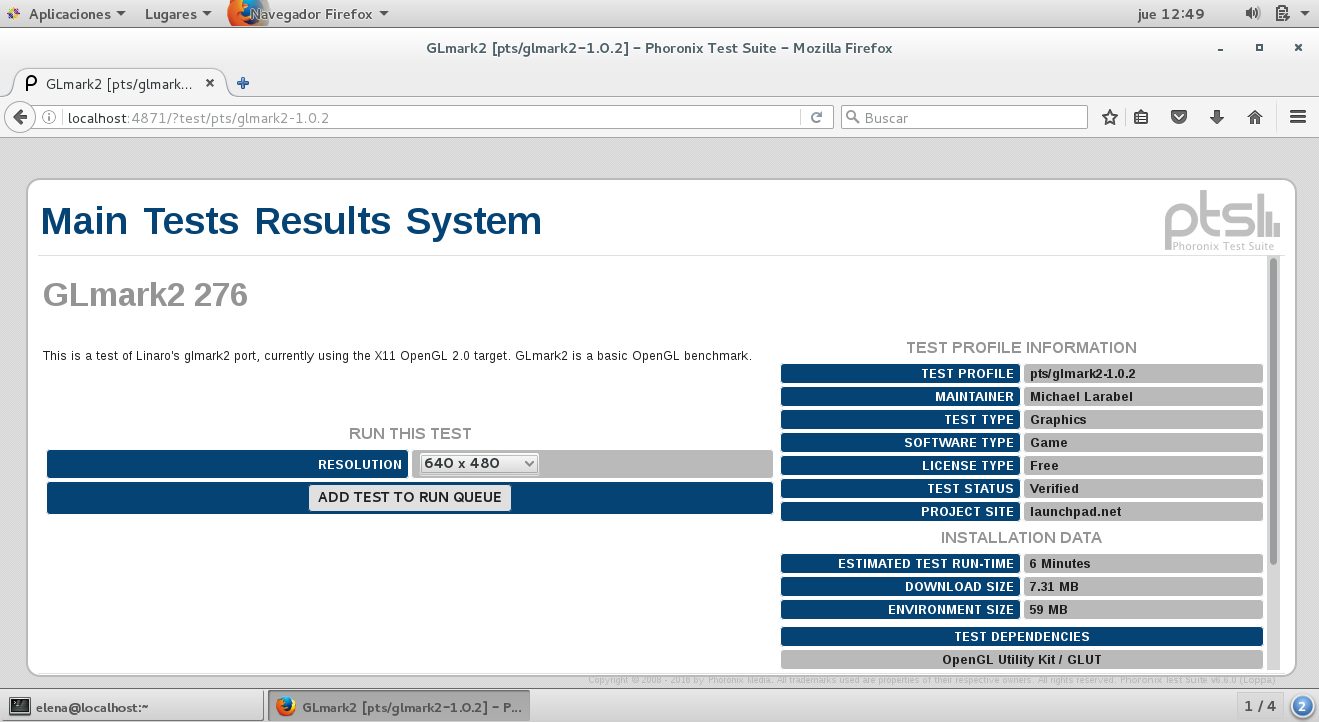
\includegraphics[width=14.7cm]{./img/ejercicio1_11.png} 	
	\caption{CentOS, Phoronix Suite, ejecución de benchmark GLmark2.} \label{fig:ejercicio1_11}
\end{figure}

\begin{figure}[H] 
	\centering
	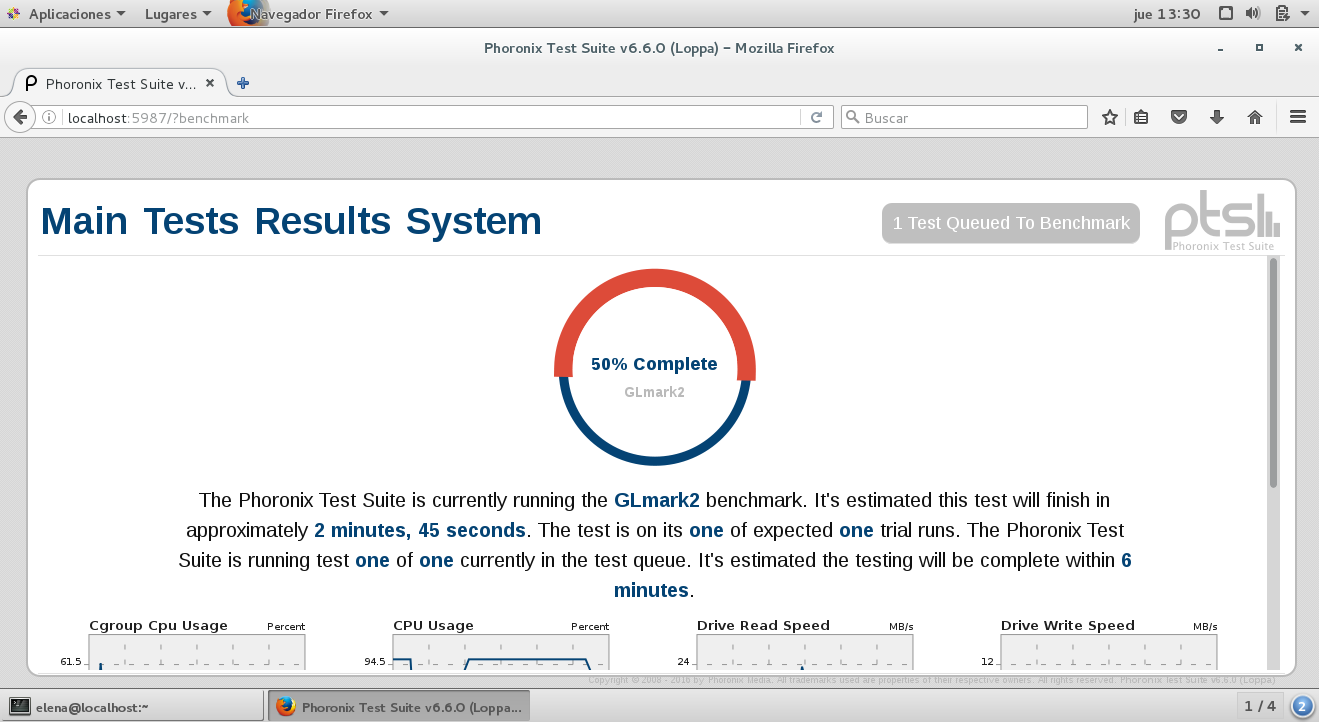
\includegraphics[width=14.7cm]{./img/ejercicio1_12.png} 	
	\caption{CentOS, Phoronix Suite, ejecución de benchmark GLmark2.} \label{fig:ejercicio1_12}
\end{figure}

\begin{figure}[H] 
	\centering
	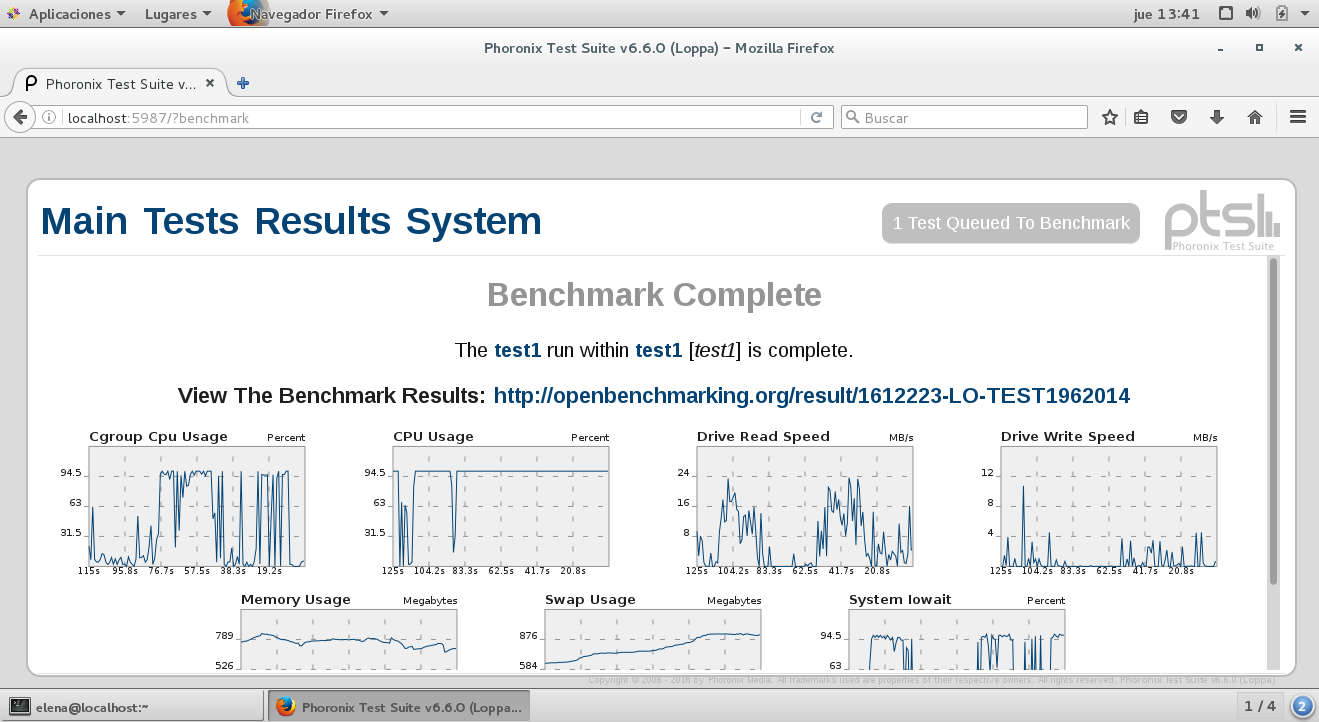
\includegraphics[width=14.7cm]{./img/ejercicio1_13.png} 	
	\caption{CentOS, Phoronix Suite, benchmark GLmark2 finalizado.} \label{fig:ejercicio1_13}
\end{figure}

\begin{figure}[H] 
	\centering
	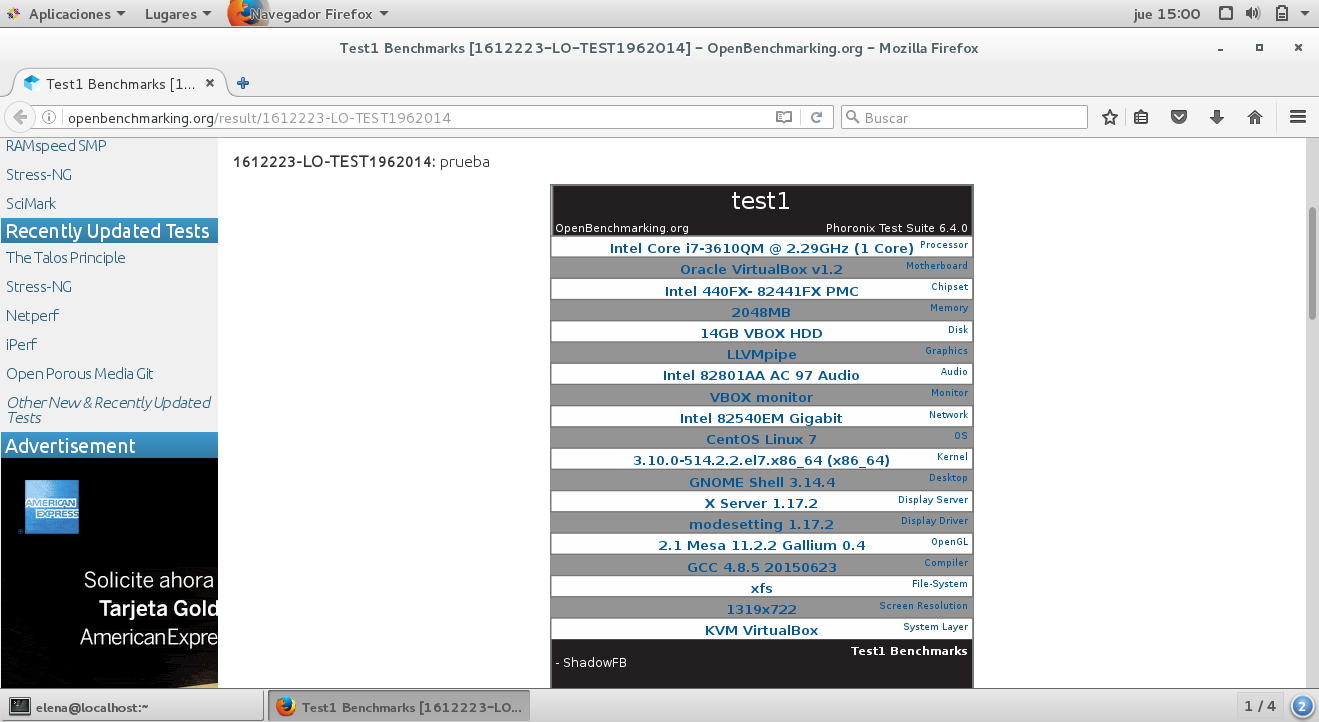
\includegraphics[width=14.7cm]{./img/ejercicio1_14.png} 	
	\caption{CentOS, Phoronix Suite, resultado de benchmark GLmark2.} \label{fig:ejercicio1_14}
\end{figure}

\begin{figure}[H] 
	\centering
	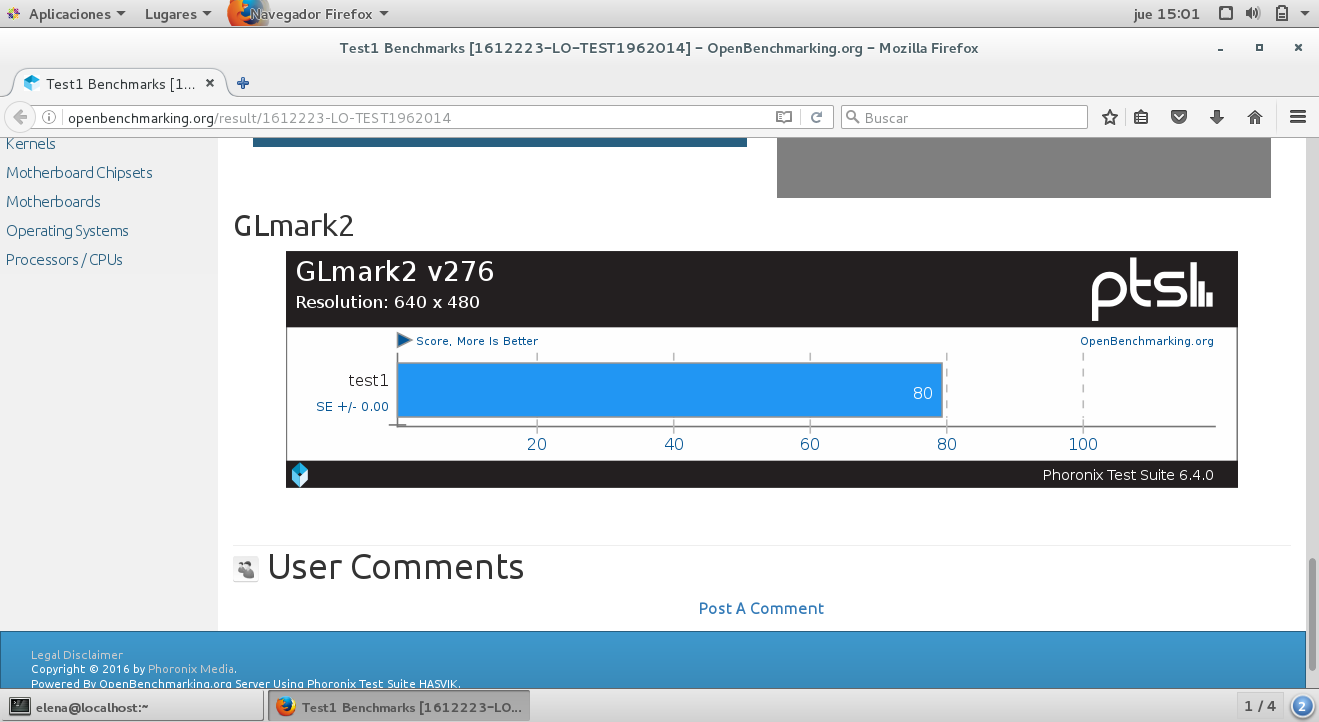
\includegraphics[width=14.7cm]{./img/ejercicio1_15.png} 	
	\caption{CentOS, Phoronix Suite, resultado de benchmark GLmark2.} \label{fig:ejercicio1_15}
\end{figure}

%----------------------------------------------------------------------------------------
%	Cuestión 2
%----------------------------------------------------------------------------------------

\section{Cuestión 2:}

\subsection{De los parámetros que le podemos pasar al comando ¿Qué significa -c 5? ¿y -n 100? Monitorice la ejecución de ab contra alguna máquina (cualquiera) ¿cuántas ``tareas'' crea ab en el cliente?}



%----------------------------------------------------------------------------------------
%	Cuestión 3
%----------------------------------------------------------------------------------------

\section{Cuestión 3:}

\subsection{Ejecute ab contra a las tres máquinas virtuales (desde el SO anfitrión a las máquina virtuales de la red local) una a una (arrancadas por separado).¿Cuál es la que proporciona mejores resultados? Muestre y coméntelos. (Use como máquina de referencia Ubuntu Server para la comparativa).}



%----------------------------------------------------------------------------------------
%  Cuestión opcional 1:
%----------------------------------------------------------------------------------------

\section{Cuestión opcional 1:}

\subsection{¿Qué es Scala? Instale Gatling y pruebe los escenarios por defecto.}


%----------------------------------------------------------------------------------------
%	Cuestión 4
%----------------------------------------------------------------------------------------

\section{Cuestión 4:}

\subsection{Instale y siga el tutorial en http://jmeter.apache.org/usermanual/build-web-test-plan.html \cite{ejer4} realizando capturas de pantalla y comentándolas. En vez de usar la web de jmeter, haga el experimento usando sus máquinas virtuales ¿coincide con los resultados de ab?}




%----------------------------------------------------------------------------------------
%	Cuestión 5
%----------------------------------------------------------------------------------------

\section{Cuestión 5:}
\subsection{Programe un benchmark usando el lenguaje que desee. El benchmark debe incluir:}

\begin{enumerate}
	\item \textbf{Objetivo del benchmark.}
	\item \textbf{Métricas (unidades, variables, puntuaciones, etc.).}
	\item \textbf{Instrucciones para su uso.}
	\item \textbf{Ejemplo de uso analizando los resultados.}
\end{enumerate}

\textbf{Tenga en cuenta que puede comparar varios gestores de BD, lenguajes de programación web (tiempos de ejecución, gestión de memoria, ...), duración de la batería, servidor DNS, etc. . Alternativamente, puede descargar alguno de algún repositorio en github y modificarlo según sus necesidades.}









%----------------------------------------------------------------------------------------
%  Extra
%----------------------------------------------------------------------------------------

%\section{Tareas extra:}




%------------------------------------------------

\bibliography{citas} %archivo citas.bib que contiene las entradas 
\bibliographystyle{plain} % hay varias formas de citar

\end{document}
